\subsubsection*{Parton level comparisons}

\begin{table}
\begin{center} 
\begin{tabular}{ c | c | c }
 $\mu = \mu_{\rm fix}$ / $\sigma_{\rm LO}^{\rm EW}$ [fb] & ${\rm p} {\rm p} \to {\rm e}^+  \nu_{\rm e}  \mu^+ \mu^- {\rm j} {\rm j}$  & ${\rm p} {\rm p} \to {\rm e}^-  \bar \nu_{\rm e}  \mu^+ \mu^- {\rm j} {\rm j}$  \\
  \hline\hline
{\sc MG5\_aMC}        & $XX$  & $XX$   \\
  {\sc MoCaNLO}+{\sc Recola}             & $0.28496(6)$  & $0.16718(3)$  \\
{\sc Sherpa}        & $0.285(5)$  & $0.1664(9)$   \\
{\sc VBFNLO}        & $XX$  & $XX$   \\
  \hline
\end{tabular}
\end{center}
\caption{
Fiducial cross sections at LO for the process ${\rm p}{\rm p}\to{\rm e}^+\nu_{\rm e}\mu^+\mu^-{\rm j}{\rm j}$ and ${\rm p}{\rm p}\to{\rm e}^-\bar\nu_{\rm e}\mu^+\mu^-{\rm j}{\rm j}$ at order $\mathcal{O} (\alpha^6)$.
The predictions are expressed in fb and are for the LHC running at a centre-of-mass energy of $\sqrt{s}=13 {\rm TeV}$.
The scale used in the simulations is $\mu = \mu_{\rm fix} = M_W$.
The integration errors of the last digits are given in parentheses.}
\label{table:xsectLOfix}
\end{table}

\begin{table}
\begin{center} 
\begin{tabular}{ c | c | c }
 $\mu = \mu_{\rm dyn}$ / $\sigma_{\rm LO}^{\rm EW}$ [fb] & ${\rm p} {\rm p} \to {\rm e}^+  \nu_{\rm e}  \mu^+ \mu^- {\rm j} {\rm j}$  & ${\rm p} {\rm p} \to {\rm e}^-  \bar \nu_{\rm e}  \mu^+ \mu^- {\rm j} {\rm j}$  \\
  \hline\hline
{\sc MG5\_aMC}        & $XX$  & $XX$   \\
  {\sc MoCaNLO}+{\sc Recola}             & $0.25416(6)$  & $0.15003(3)$  \\
{\sc Sherpa}        & $0.2573(3)$  & $0.1499(2)$   \\
{\sc VBFNLO}        & $XX$  & $XX$   \\
  \hline
\end{tabular}
\end{center}
\caption{
Fiducial cross sections at LO for the process ${\rm p}{\rm p}\to{\rm e}^+\nu_{\rm e}\mu^+\mu^-{\rm j}{\rm j}$ and ${\rm p}{\rm p}\to{\rm e}^-\bar\nu_{\rm e}\mu^+\mu^-{\rm j}{\rm j}$ at order $\mathcal{O} (\alpha^6)$.
The predictions are expressed in fb and are for the LHC running at a centre-of-mass energy of $\sqrt{s}=13 {\rm TeV}$.
The scale used in the simulations is $\mu = \mu_{\rm dyn} = {\rm Max}\left[p_{\rm T, j}\right]$.
The integration errors of the last digits are given in parentheses.}
\label{table:xsectLOdyn}
\end{table}

\subsubsection*{Comparisons after parton shower}

Figures~\ref{vbs_fig_shower_1a} and \ref{vbs_fig_shower_1b} show a comparison of results obtained with different
generators for ${\rm p} {\rm p} \to {\rm e}^+  \nu_{\rm e}  \mu^+ \mu^- {\rm j} {\rm j}$ at LO with fixed scaled $\mu =
M_W$.
Figures~\ref{vbs_fig_shower_2a} and \ref{vbs_fig_shower_2b} show the same distribution for \MGAMC with different scale
choices, either dynamic or fixed with value equal to $M_W$ and $M_Z$.
Finally in Figures~\ref{vbs_fig_shower_3a},\ref{vbs_fig_shower_3b},\ref{vbs_fig_shower_4a} and \ref{vbs_fig_shower_4b} a
comparison of results for ${\rm p} {\rm p} \to {\rm e}^-  \nu_{\rm e}  \mu^+ \mu^- {\rm j} {\rm j}$ and ${\rm p} {\rm p}
\to {\rm e}^-  \nu_{\rm e}  \mu^+ \mu^- {\rm j} {\rm j}$ is shown for 
different generators and different scale values, dynamic or fixed.    

\begin{figure}[htbp]
\begin{center}
   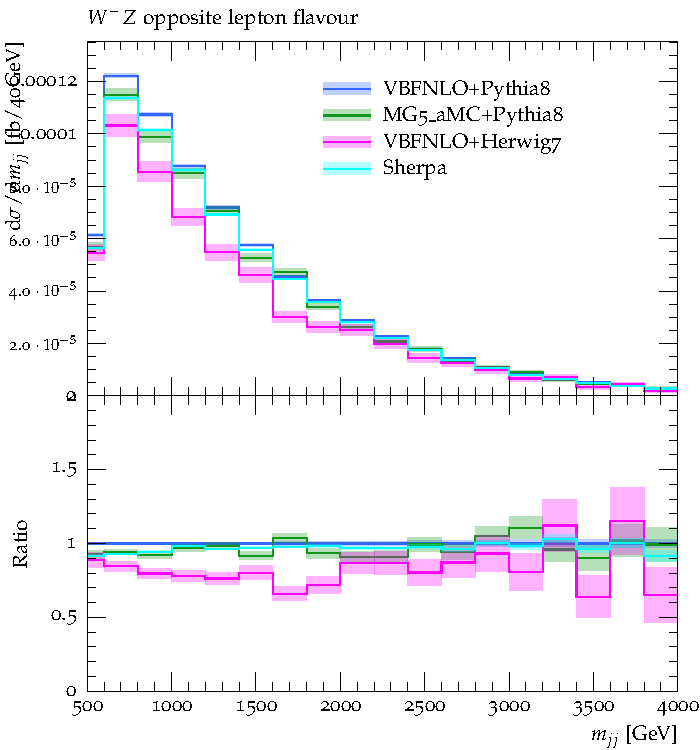
\includegraphics[scale=0.65]{figs/VBFNLO_WmZ_OF_mjj}
   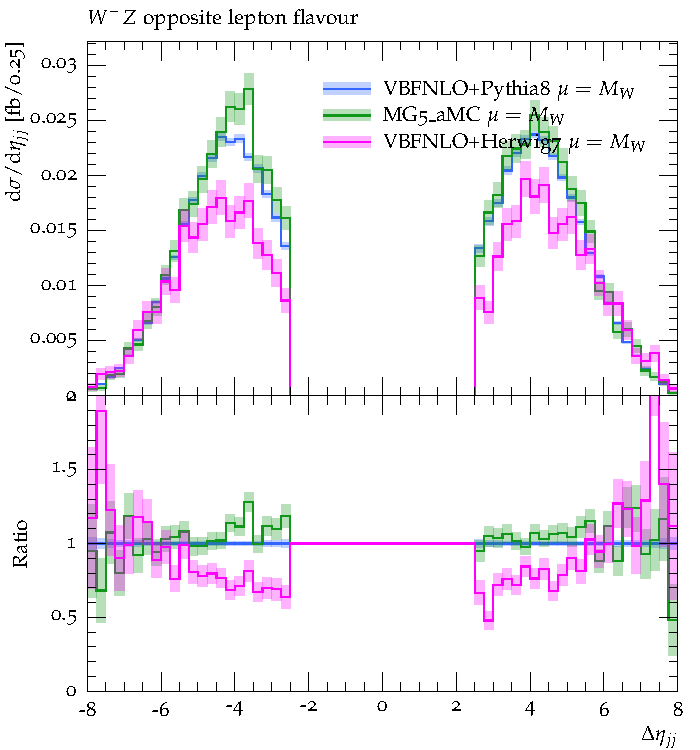
\includegraphics[scale=0.65]{figs/VBFNLO_WmZ_OF_dEtajj}
   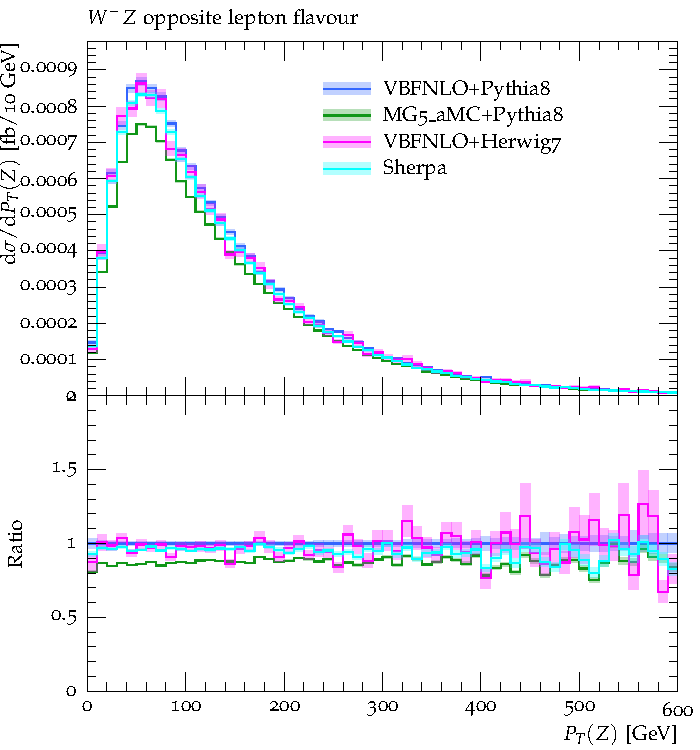
\includegraphics[scale=0.65]{figs/VBFNLO_WmZ_OF_ZPt}
   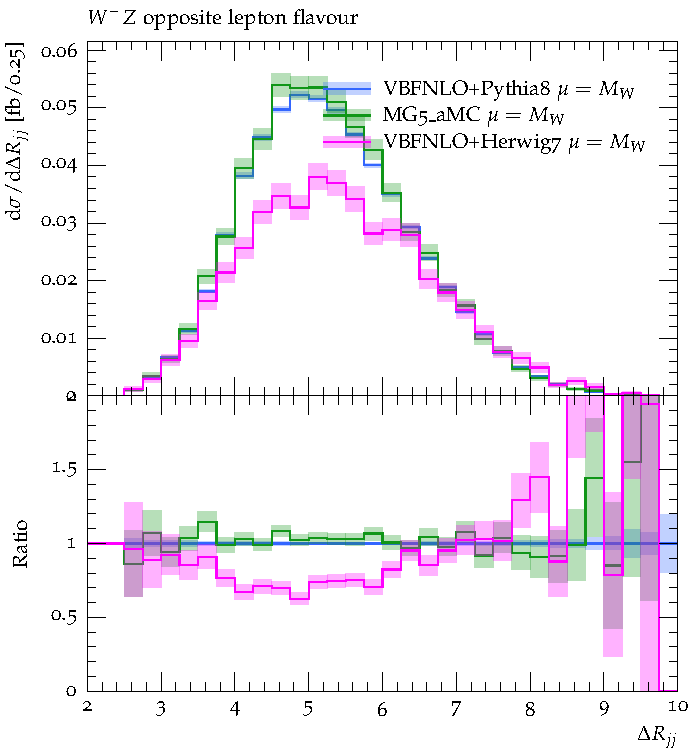
\includegraphics[scale=0.65]{figs/VBFNLO_WmZ_OF_dRjj}
\caption{Differential distributions at a centre-of-mass energy $\sqrt{s}=13{\rm TeV}$ at the LHC for ${\rm p} {\rm p}
  \to {\rm e}^-  \nu_{\rm e}  \mu^+ \mu^- {\rm j} {\rm j}$ at LO with fixed scaled $\mu = M_W$: 
                invariant mass of the two jets~(top left),
                rapidity separation between the two jets~(top right)
                transverse momentum of the anti-muon--muon~(bottom left), and
                distance between the two jets~(bottom right).}
\label{vbs_fig_shower_1a}
\end{center}
\end{figure}

\begin{figure}[htbp]
\begin{center}
   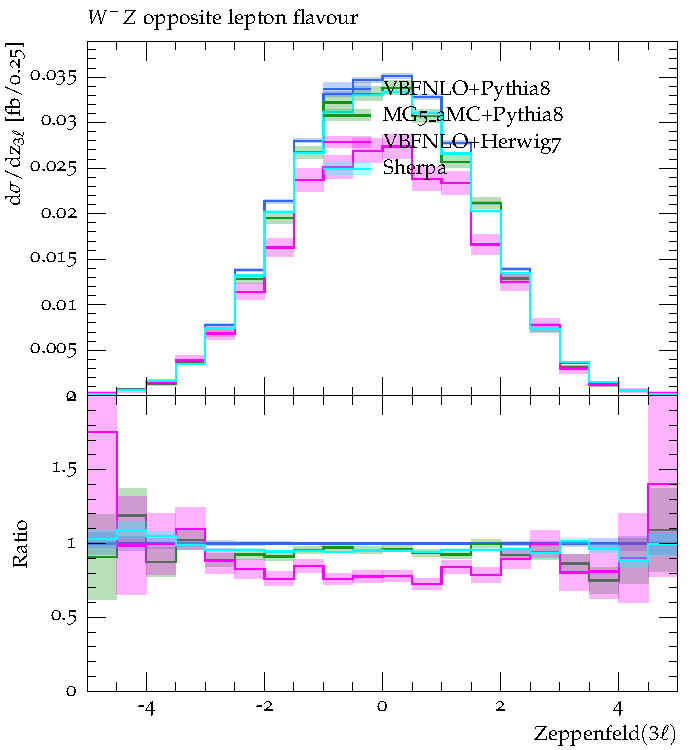
\includegraphics[scale=0.65]{figs/VBFNLO_WmZ_OF_zep3l}
   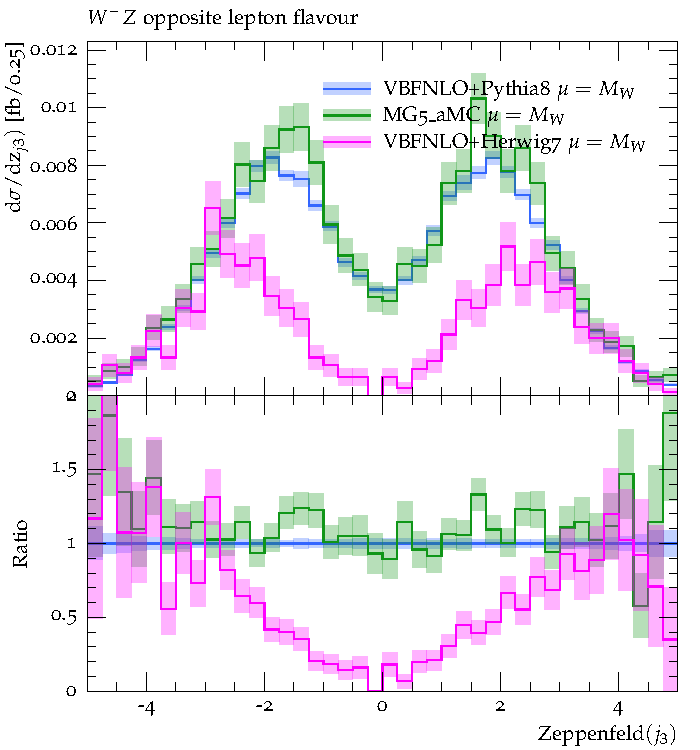
\includegraphics[scale=0.65]{figs/VBFNLO_WmZ_OF_zepj3}
   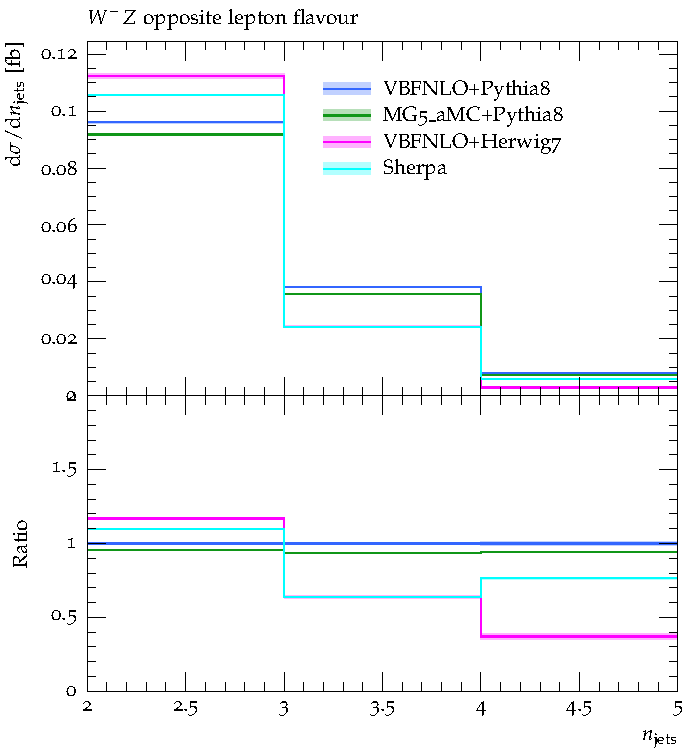
\includegraphics[scale=0.65]{figs/VBFNLO_WmZ_OF_nJets}
\caption{Differential distributions at a centre-of-mass energy $\sqrt{s}=13{\rm TeV}$ at the LHC for ${\rm p} {\rm p}
  \to {\rm e}^-  \nu_{\rm e}  \mu^+ \mu^- {\rm j} {\rm j}$ at LO with fixed scaled $\mu = M_W$: 
                Zeppenfeld variable for the three leptons~(top left),
                Zeppenfeld variable for the third jet~(top right)
                number of jets~(bottom).}
\label{vbs_fig_shower_1b}
\end{center}
\end{figure}


\begin{figure}[htbp]
\begin{center}
   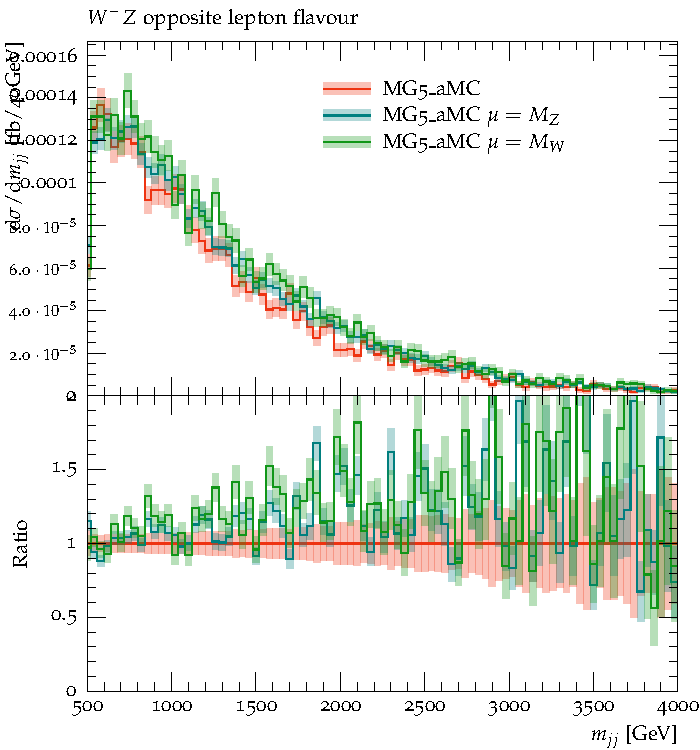
\includegraphics[scale=0.65]{figs/MG_WmZ_OF_mjj}
   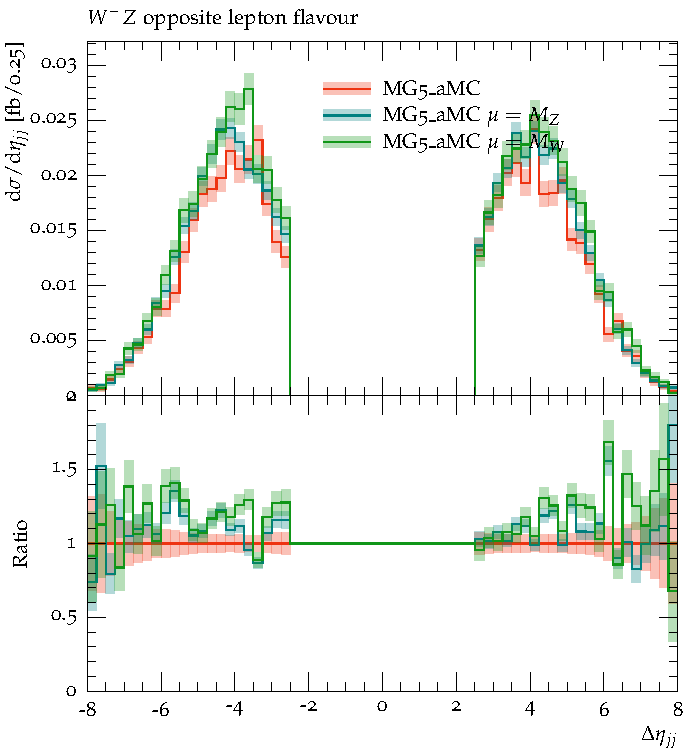
\includegraphics[scale=0.65]{figs/MG_WmZ_OF_dEtajj}
   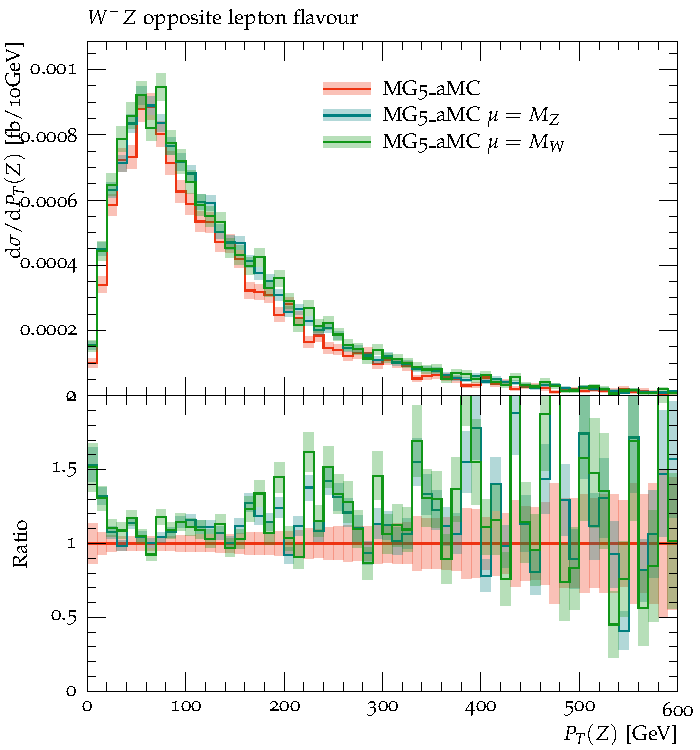
\includegraphics[scale=0.65]{figs/MG_WmZ_OF_ZPt}
   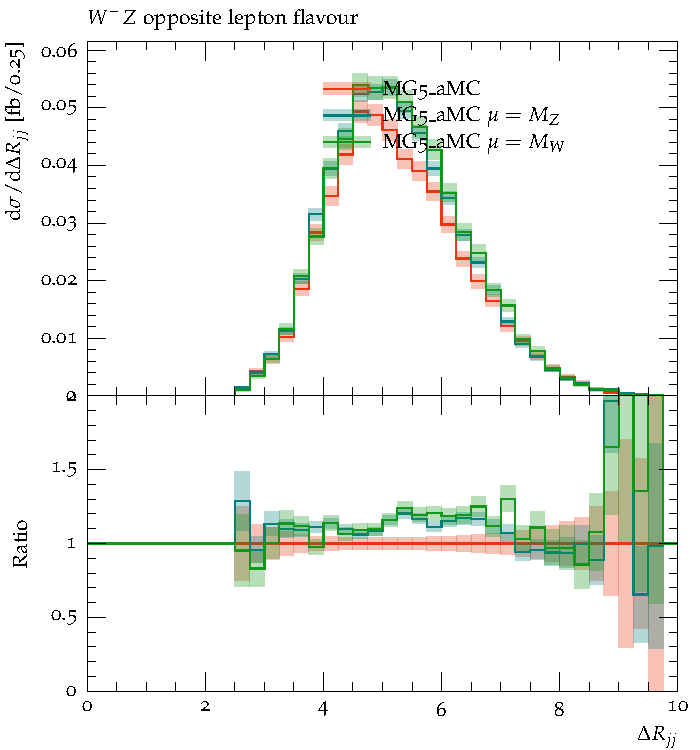
\includegraphics[scale=0.65]{figs/MG_WmZ_OF_dRjj}
\caption{Differential distributions at a centre-of-mass energy $\sqrt{s}=13{\rm TeV}$ at the LHC for ${\rm p} {\rm p}
  \to {\rm e}^-  \nu_{\rm e}  \mu^+ \mu^- {\rm j} {\rm j}$ at LO with fixed and dynamic scale values: 
                invariant mass of the two jets~(top left),
                rapidity separation between the two jets~(top right)
                transverse momentum of the anti-muon--muon~(bottom left), and
                distance between the two jets~(bottom right).}
\label{vbs_fig_shower_2a}
\end{center}
\end{figure}

\begin{figure}[htbp]
\begin{center}
   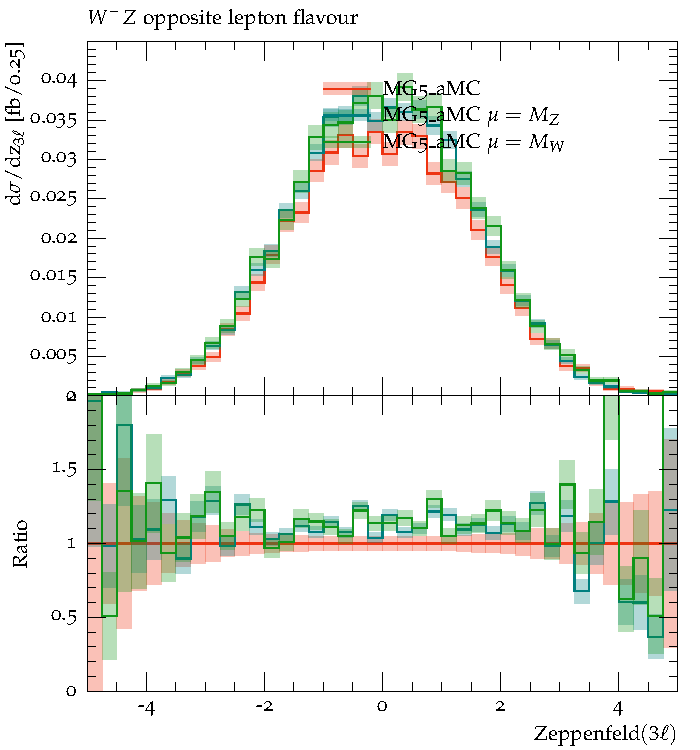
\includegraphics[scale=0.65]{figs/MG_WmZ_OF_zep3l}
   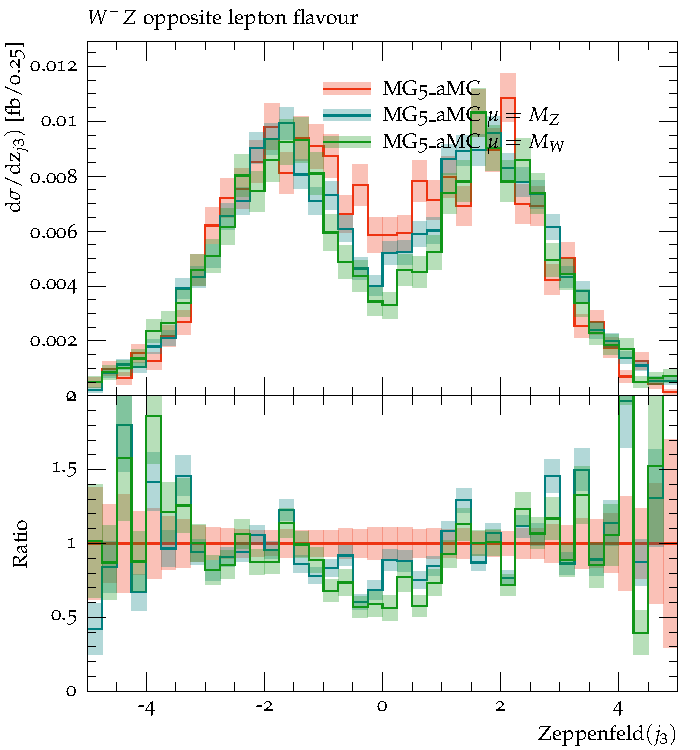
\includegraphics[scale=0.65]{figs/MG_WmZ_OF_zepj3}
   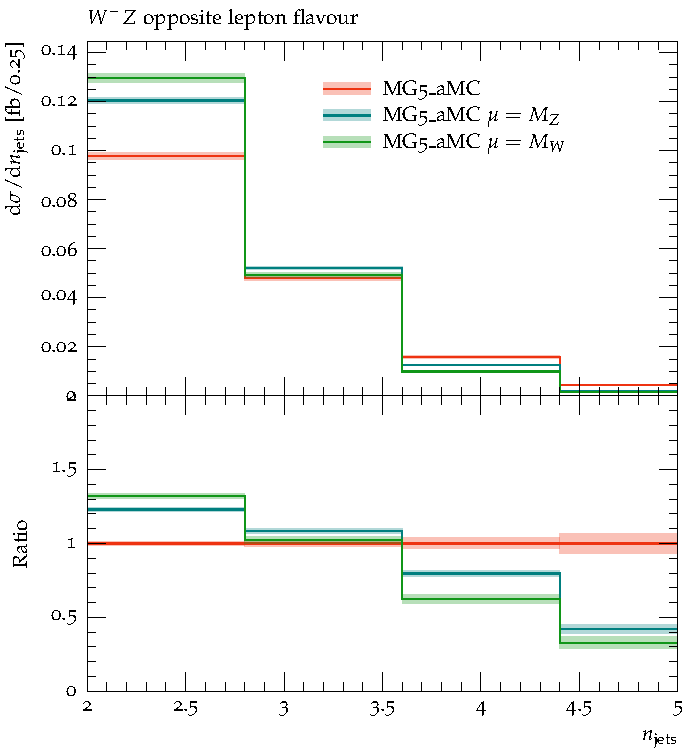
\includegraphics[scale=0.65]{figs/MG_WmZ_OF_nJets}
\caption{Differential distributions at a centre-of-mass energy $\sqrt{s}=13{\rm TeV}$ at the LHC for ${\rm p} {\rm p}
  \to {\rm e}^-  \nu_{\rm e}  \mu^+ \mu^- {\rm j} {\rm j}$ at LO with fixed and dynamic scale values:  
                Zeppenfeld variable for the three leptons~(top left),
                Zeppenfeld variable for the third jet~(top right)
                number of jets~(bottom).}
\label{vbs_fig_shower_2b}
\end{center}
\end{figure}

\begin{figure}[htbp]
\begin{center}
   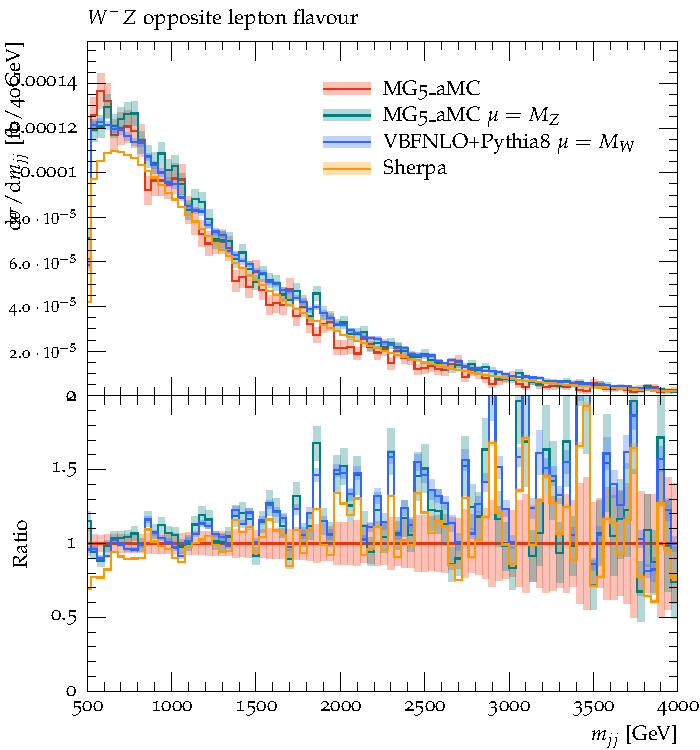
\includegraphics[scale=0.65]{figs/WmZ_OF_mjj}
   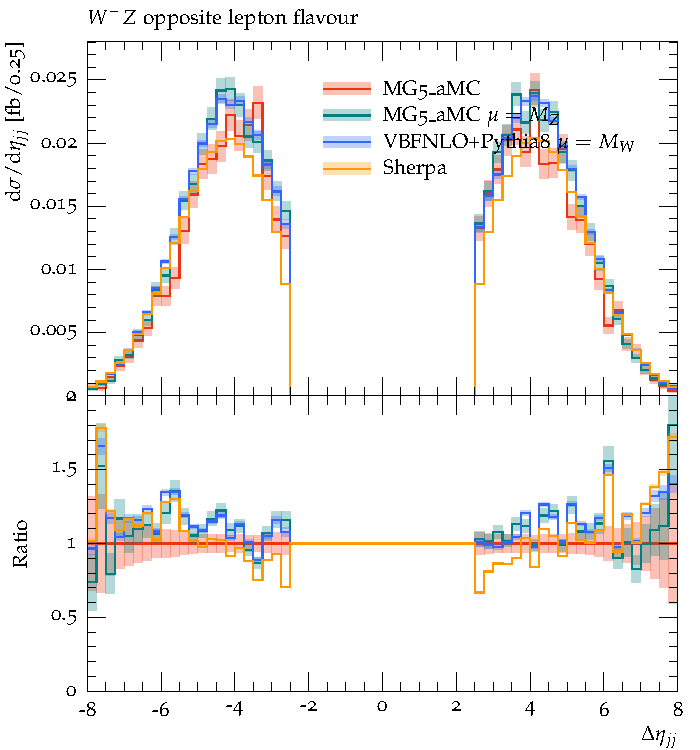
\includegraphics[scale=0.65]{figs/WmZ_OF_dEtajj}
   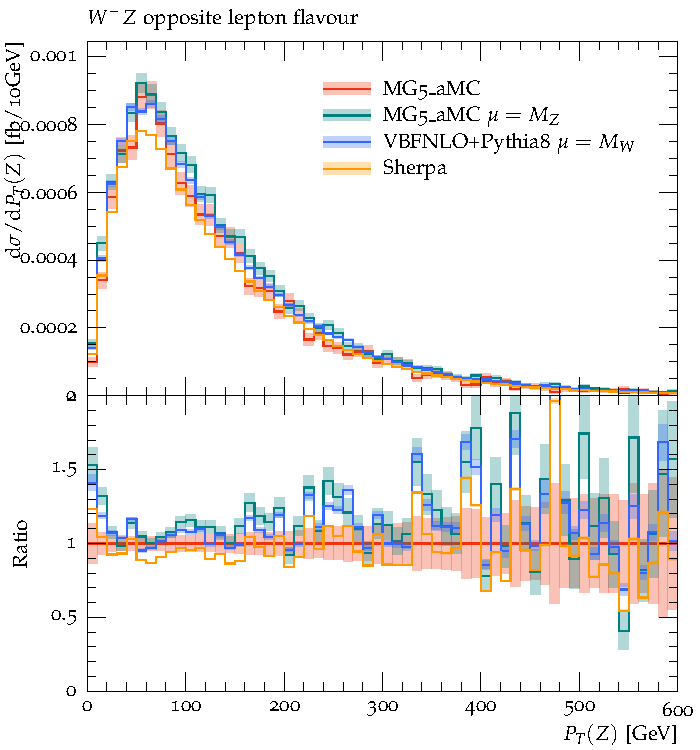
\includegraphics[scale=0.65]{figs/WmZ_OF_ZPt}
   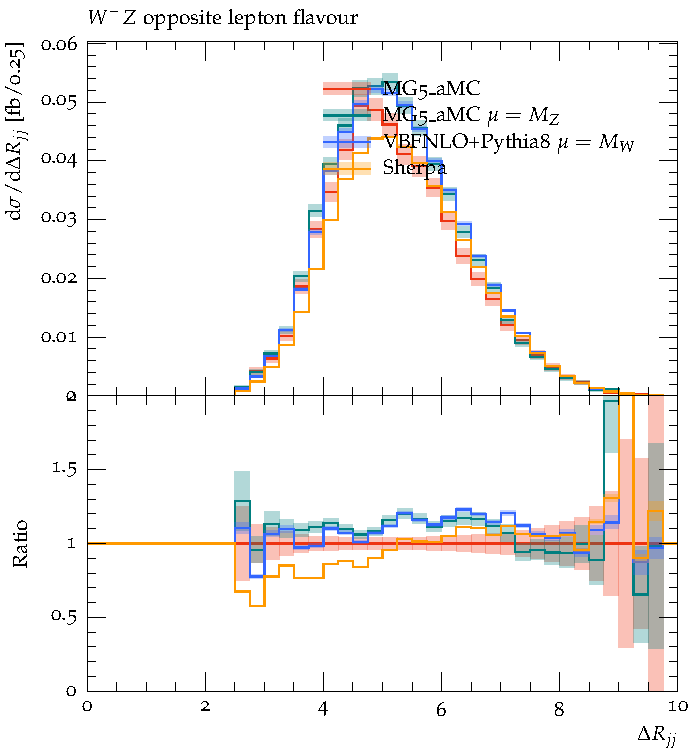
\includegraphics[scale=0.65]{figs/WmZ_OF_dRjj}
\caption{Differential distributions at a centre-of-mass energy $\sqrt{s}=13{\rm TeV}$ at the LHC for ${\rm p} {\rm p}
  \to {\rm e}^-  \nu_{\rm e}  \mu^+ \mu^- {\rm j} {\rm j}$ at LO with fixed and dynamic scale values:  
                invariant mass of the two jets~(top left),
                rapidity separation between the two jets~(top right)
                transverse momentum of the anti-muon--muon~(bottom left), and
                distance between the two jets~(bottom right).}
\label{vbs_fig_shower_3a}
\end{center}
\end{figure}

\begin{figure}[htbp]
\begin{center}
   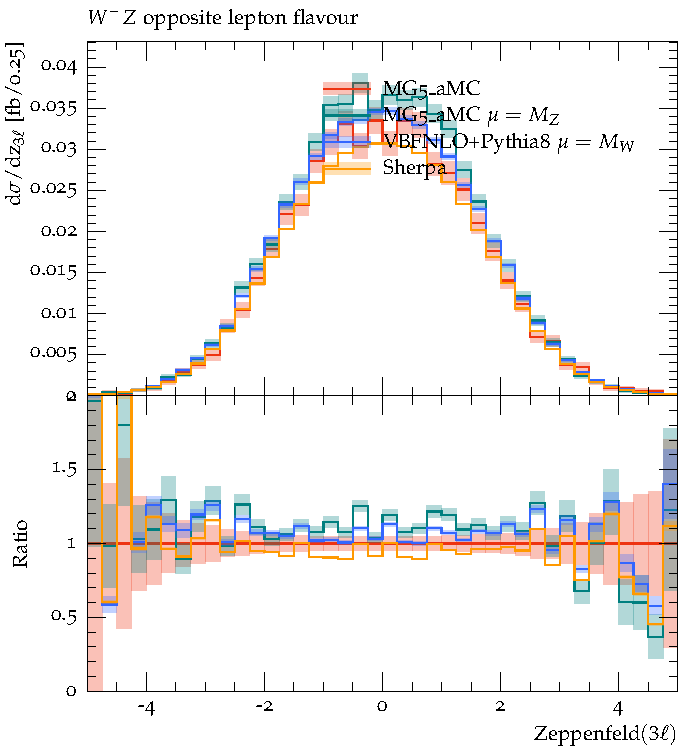
\includegraphics[scale=0.65]{figs/WmZ_OF_zep3l}
   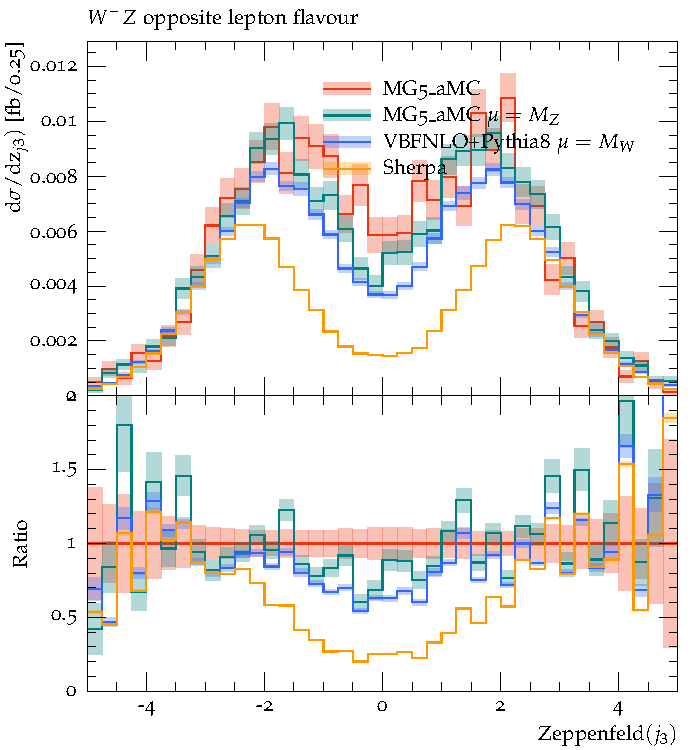
\includegraphics[scale=0.65]{figs/WmZ_OF_zepj3}
   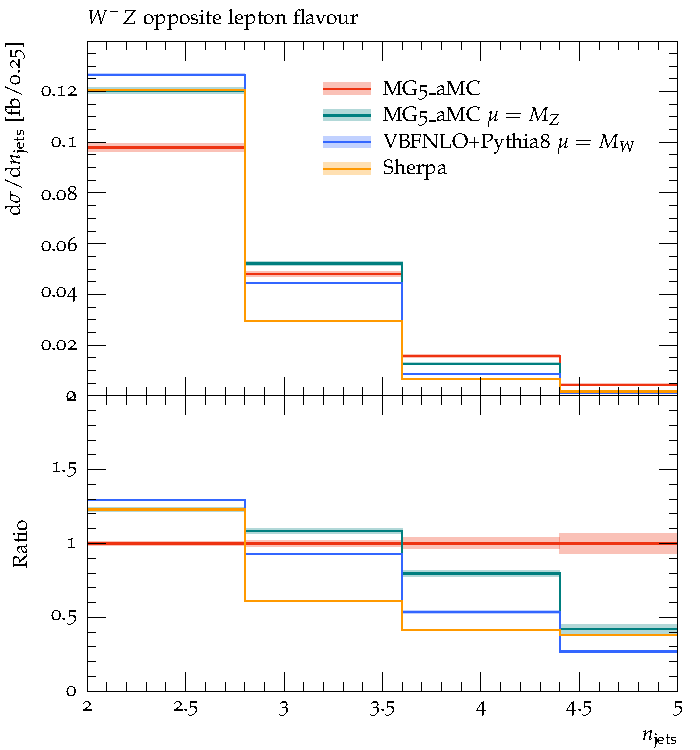
\includegraphics[scale=0.65]{figs/WmZ_OF_nJets}
\caption{Differential distributions at a centre-of-mass energy $\sqrt{s}=13{\rm TeV}$ at the LHC for ${\rm p} {\rm p} \to {\rm e}^-  \nu_{\rm e}  \mu^+ \mu^- {\rm j} {\rm j}$ at LO with fixed and dynamic scale values: 
                Zeppenfeld variable for the three leptons~(top left),
                Zeppenfeld variable for the third jet~(top right)
                number of jets~(bottom).}
\label{vbs_fig_shower_3b}
\end{center}
\end{figure}

\begin{figure}[htbp]
\begin{center}
   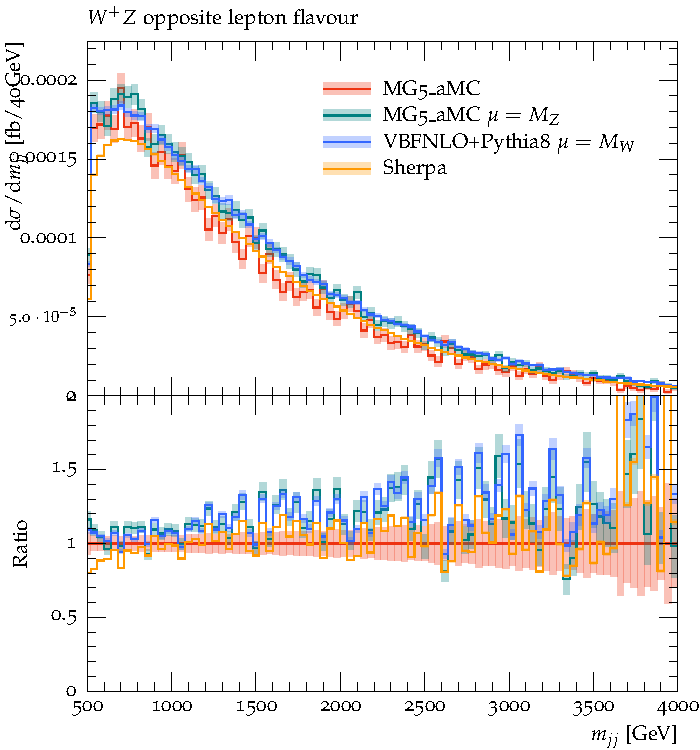
\includegraphics[scale=0.65]{figs/WpZ_OF_mjj}
   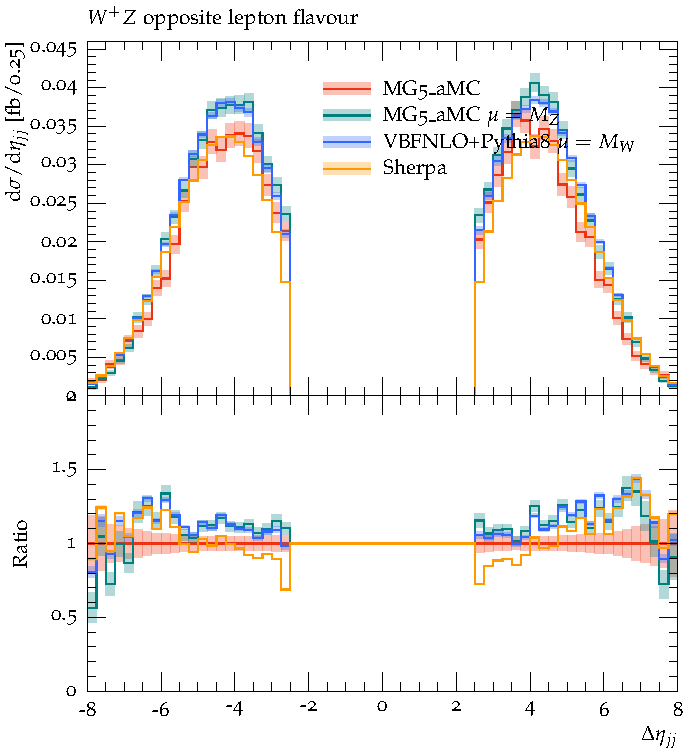
\includegraphics[scale=0.65]{figs/WpZ_OF_dEtajj}
   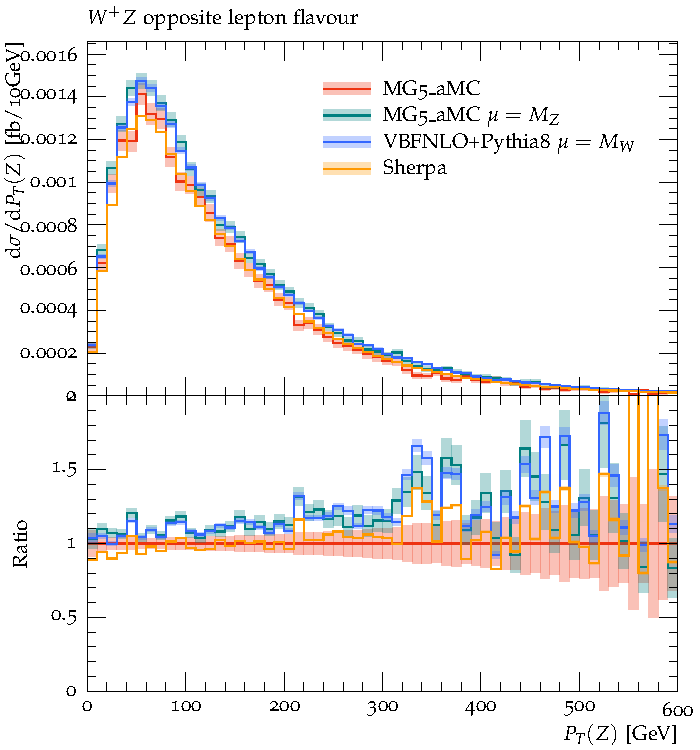
\includegraphics[scale=0.65]{figs/WpZ_OF_ZPt}
   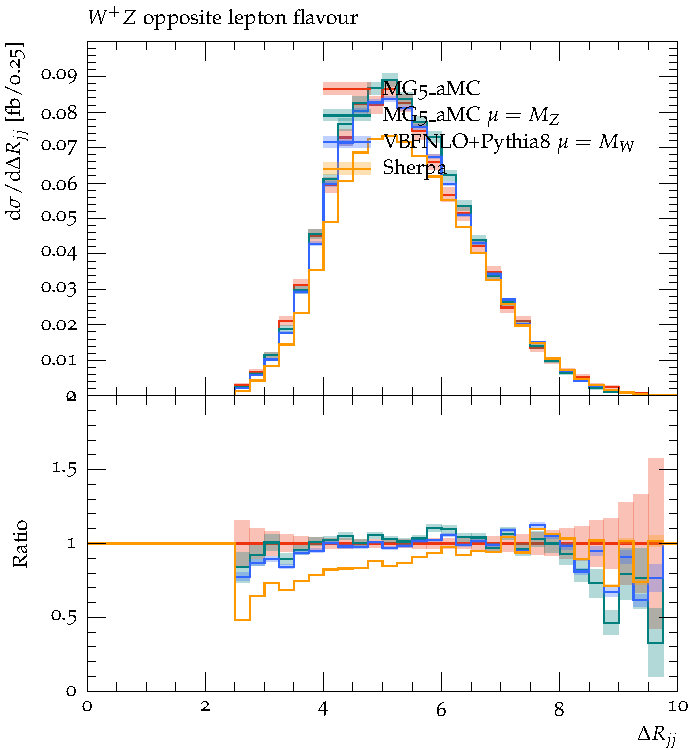
\includegraphics[scale=0.65]{figs/WpZ_OF_dRjj}
\caption{Differential distributions at a centre-of-mass energy $\sqrt{s}=13{\rm TeV}$ at the LHC for ${\rm p} {\rm p}
  \to {\rm e}^+  \nu_{\rm e}  \mu^+ \mu^- {\rm j} {\rm j}$ at LO with fixed and dynamic scale values:  
                invariant mass of the two jets~(top left),
                rapidity separation between the two jets~(top right)
                transverse momentum of the anti-muon--muon~(bottom left), and
                distance between the two jets~(bottom right).}
\label{vbs_fig_shower_4a}
\end{center}
\end{figure}

\begin{figure}[htbp]
\begin{center}
   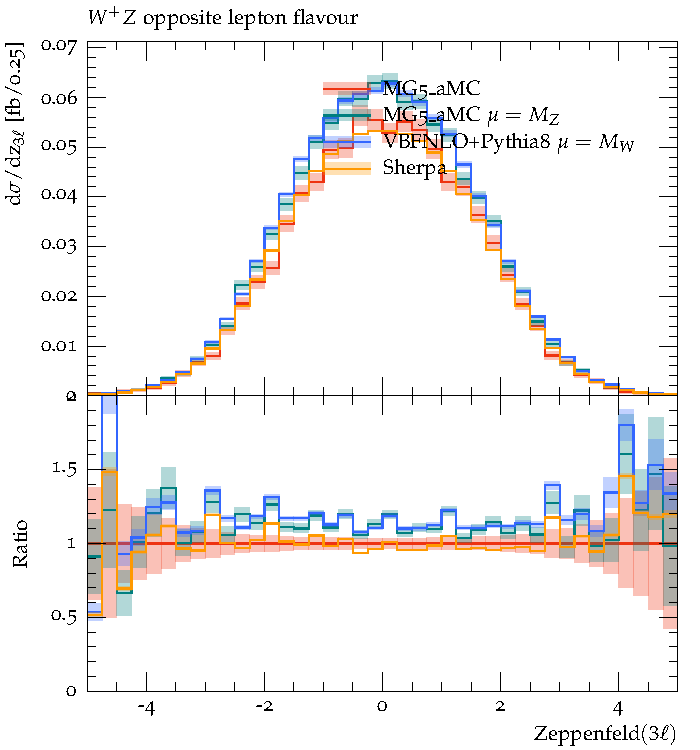
\includegraphics[scale=0.65]{figs/WpZ_OF_zep3l}
   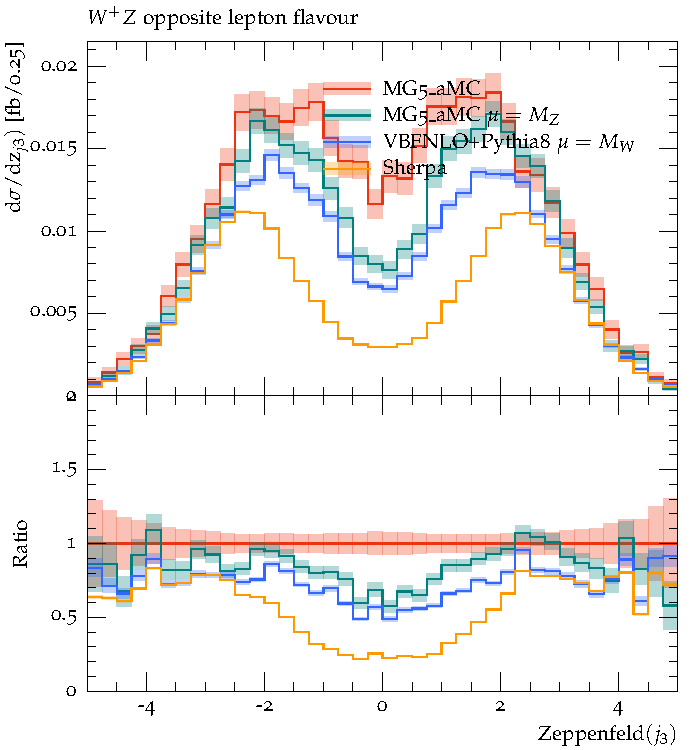
\includegraphics[scale=0.65]{figs/WpZ_OF_zepj3}
   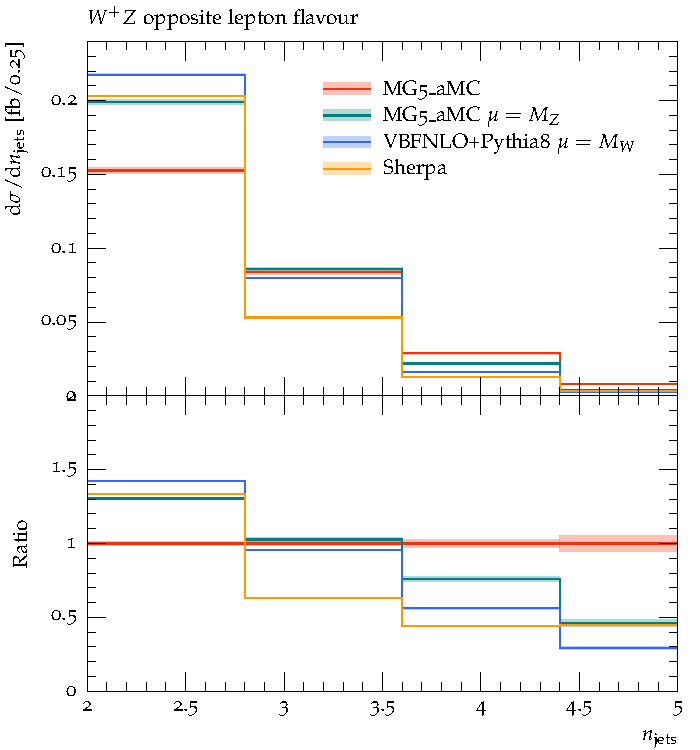
\includegraphics[scale=0.65]{figs/WpZ_OF_nJets}
\caption{Differential distributions at a centre-of-mass energy $\sqrt{s}=13{\rm TeV}$ at the LHC for ${\rm p} {\rm p} \to {\rm e}^+  \nu_{\rm e}  \mu^+ \mu^- {\rm j} {\rm j}$ at LO with fixed and dynamic scale values: 
                Zeppenfeld variable for the three leptons~(top left),
                Zeppenfeld variable for the third jet~(top right)
                number of jets~(bottom).}
\label{vbs_fig_shower_4b}
\end{center}
\end{figure}
